\documentclass{article}
\usepackage{nips10submit_e,times}
%\documentstyle[nips07submit_09,times]{article}
\usepackage[square,numbers]{natbib}
\usepackage{amsmath, epsfig}
\usepackage{amsfonts}
\usepackage{subfigure}
\usepackage{graphicx}
\usepackage{amsfonts}
\usepackage{algorithm}
\usepackage{algorithmic}
\usepackage{easybmat}
\usepackage{footmisc}
\usepackage{lscape}
\renewcommand\algorithmiccomment[1]{// \textit{#1}}
%
\newcommand{\ignore}[1]{}
\newcommand{\comment}[1]{}
\DeclareMathOperator*{\argmax}{arg\,max}

\title{Hierarchically Supervised Latent Dirichlet Allocation}
%Supervised Topic Modeling in Clinical Text}

\author{
Adler Perotte\hspace{1cm} Nicholas Bartlett \hspace{1cm} Noemie Elhadad \hspace{1cm} Frank Wood\\
Columbia University, New York, NY 10027, USA \\
\texttt{\{ajp9009@dbmi,bartlett@stat,noemie@dbmi,fwood@stat\}.columbia.edu}
%\texttt{pfau@neurotheory.columbia.edu} 
%\texttt{\{bartlett,fwood\}@stat.columbia.edu} 
}



% The \author macro works with any number of authors. There are two commands
% used to separate the names and addresses of multiple authors: \And and \AND.
%
% Using \And between authors leaves it to \LaTeX{} to determine where to break
% the lines. Using \AND forces a linebreak at that point. So, if \LaTeX{}
% puts 3 of 4 authors names on the first line, and the last on the second
% line, try using \AND instead of \And before the third author name.

\newcommand{\fix}{\marginpar{FIX}}
\newcommand{\new}{\marginpar{NEW}}
\newcommand{\X}{\mathcal{X}}


\nipsfinalcopy

\begin{document}

\maketitle

\begin{abstract}


We introduce hierarchically supervised latent Dirichlet allocation (HSLDA), a
model for hierarchically and multiply labeled bag-of-word data.  Examples of
such data include web pages and their placement in directories, product
descriptions and associated categories from product hierarchies, and free-text
clinical records and their assigned diagnosis codes. Out-of-sample label
prediction is the primary goal of this work, but improved lower-dimensional
representations of the bag-of-word data are also of interest.
%% We demonstrate HSLDA on large-scale data from clinical document labeling and
%% retail product categorization tasks. We show that leveraging the structure from
%% hierarchical labels improves out-of-sample label prediction substantially when
%% compared to models that do not. 

Our work operates within the framework of topic modeling. Our approach learns
topic models of the underlying data and labeling strategies in a joint model,
while leveraging the hierarchical structure of the labels. For the sake of
simplicity, we focus on is-a hierarchies, but the model can be
applied to other structured label spaces. Our work extends supervised latent Dirichlet
allocation (sLDA)~\cite{BleiMcAuliffe2008} to take advantage of hierarchical
supervision and proposes an efficient way to incorporate such information into the model. 
We hypothesize that the context of labels within
the hierarchy provides valuable information about labeling. Other models, such as LabeledLDA~\citep{Ramage2009}, incorporate LDA and supervision; however, none of these models leverage dependency structure in the label space.

We demonstrate our model on large, real-world datasets in the clinical and web
retail domains. We observe that hierarchical information is valuable when
incorporated into the learning and improves our primary goal of multi-label
classification. Our results show that a joint, hierarchical model outperforms a
classification with unstructured labels as well as a disjoint model, where the
topic model and the hierarchical classification are inferred
independently of each other. 

HSLDA is a model for hierarchically, multiply-labeled, bag-of-word data.  We
will refer to individual groups of bag-of-word data as documents.  Let $w_{n,d}
\in \Sigma$ be the $n$th observation in the $d$th document.  Let $\mathbf{w}_d
= \{w_{1,d},\ldots,w_{1,N_d}\}$ be the  set of $N_d$ observations in document
$d$.  Let there be $D$ such documents and let the size of the vocabulary be
$V=|\Sigma|$.  Let the set of labels be $\mathcal{L}=\left\{
  l_{1},l_{2},\ldots,l_{\left|\mathcal{L}\right|}\right\} $. Each label
$l \in \mathcal{L}$, except root, has a parent $\mathrm{pa}(l) \in \mathcal{L}$
also in the set of labels. 
 We will for exposition purposes assume that this label set has hard ``is-a''
 parent-child constraints, although this assumption can be
 relaxed at the cost of more computationally complex inference.  Such a label hierarchy forms a multiply rooted tree.  Without loss of generality we will consider a tree with a single root $r\in\mathcal{L}$.  Each document has a variable $y_{l,d} \in \{-1,1\}$ for every label which indicates whether the label is applied to document $d$ or not.   In most cases $y_{i,d}$ will be unobserved, in some cases we will be able to fix its value because of  constraints on the label hierarchy, and in the relatively minor remainder its value will be observed.  In the applications we consider, only positive label applications are observed.  


%In HSLDA, the bag-of-word document data is modeled using the LDA
%mixed-membership mixture model with global topic estimation.
In HSLDA, documents are modeled using the LDA mixed-membership mixture model
with global topic estimation. Label responses are generated using a conditional
hierarchy of probit regressors\cite{gelmanbda04}. The HSLDA graphical model is given in
Figure~\ref{fig:graphical_model}. In the model, $K$ is the number of LDA
``topics'' (distributions over the elements of $\Sigma$), $\boldsymbol\phi_k$
is a distribution over ``words,'' $\boldsymbol\theta_d$ is a document-specific
distribution over topics, and $\boldsymbol\beta$ is a global distribution over
topics.
%% , Dir$_{K}(\cdot)$ is a $K$-dimensional Dirichlet distribution,
%% $\mathcal{N}_{K}(\cdot)$ is the $K$-dimensional Normal distribution,
%% $\mathbf{I}_{K}$ is the $K$ dimensional identity matrix,  $\mathbf{1}_d$ is the
%% $d$-dimensional vector of all ones, and $\mathbb{I}(\cdot)$ is an indicator
%% function that takes the value $1$ if its argument is true and $0$ otherwise. 

\begin{figure}[t]
%tbp] %  figure placement: here, top, bottom, or page
 \centering 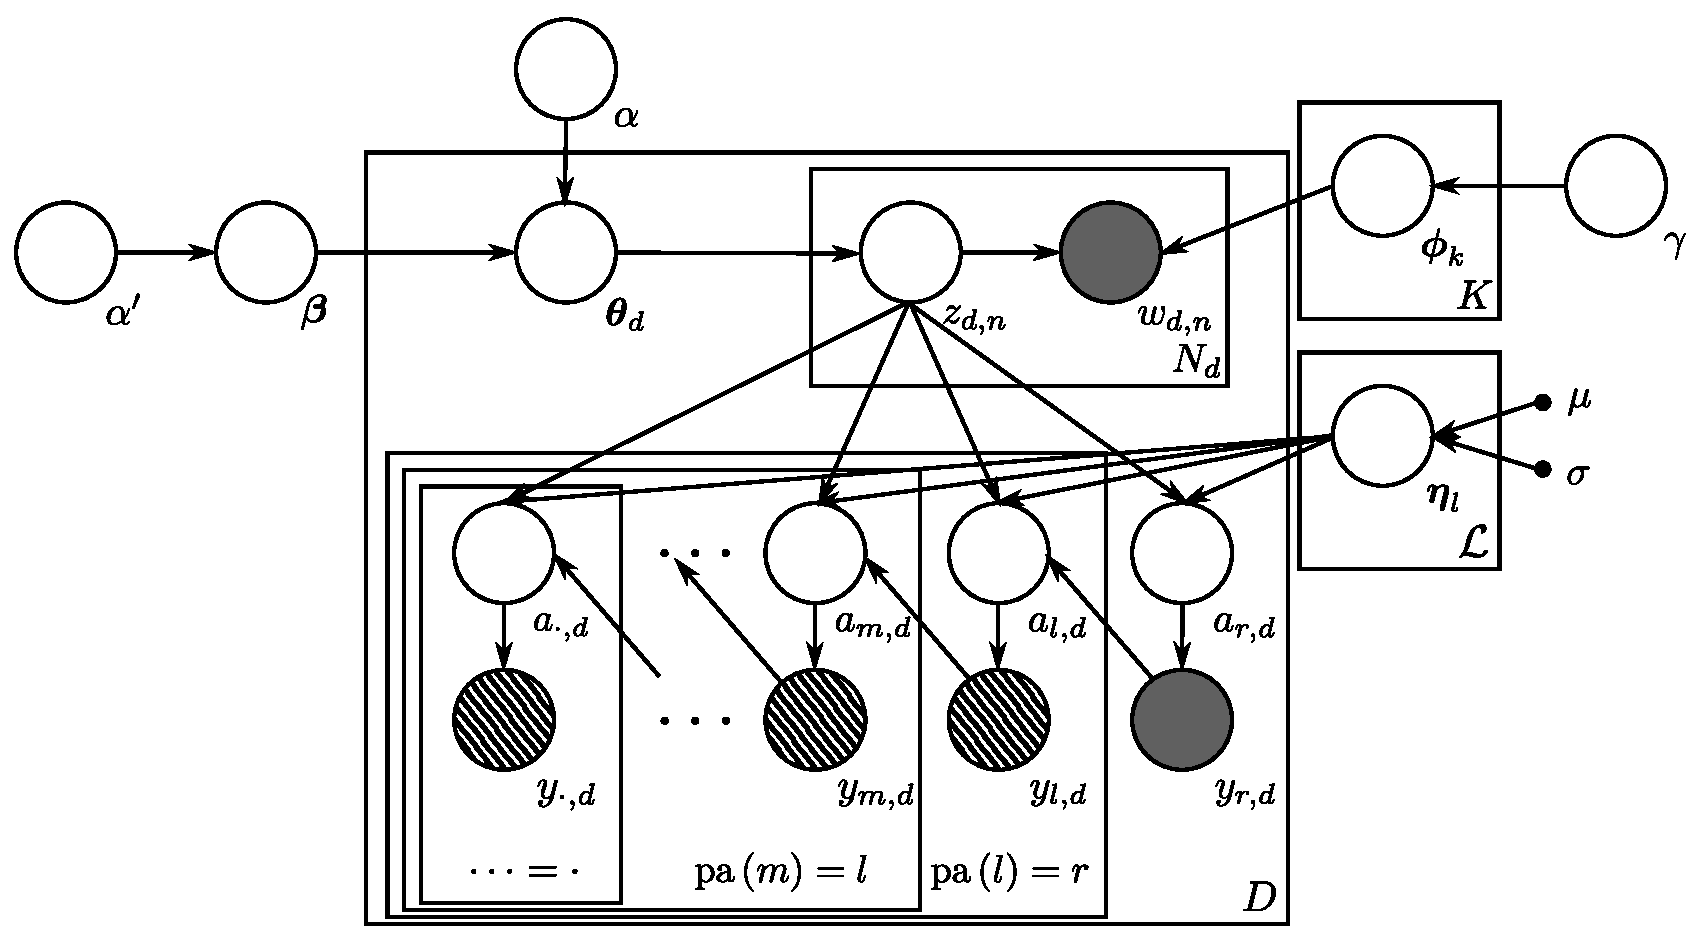
\includegraphics[scale=0.25]{Graphical_Model-final} \caption{HSLDA graphical model}


\label{fig:graphical_model} 
\end{figure}


Posterior inference in HSLDA was performed using Gibbs sampling and Markov chain Monte Carlo.  Note that, like in collapsed Gibbs samplers for LDA \cite{Griffiths04}, we have analytically marginalized out the parameters $\boldsymbol{\phi}_{1:K}$
and $\boldsymbol{\theta}_{1:D}$. HSLDA also employs a hierarchical Dirichlet prior over topic assignments (i.e.,~$\boldsymbol\beta$ is estimated from data rather than assumed to be symmetric).  This has been shown to improve the quality and stability of inferred topics \citep{WallachMiMc2009}. The hyperparameters $\alpha$, $\alpha^{\prime}$, and $\gamma$ are
%given broad ${\rm Gamma}(1,1000)$ prior distributions and 
sampled
using Metropolis-Hastings. 


We applied HSLDA to data from two domains: predicting medical
diagnosis codes from hospital discharge summaries and predicting product
categories from Amazon.com product descriptions. The clinical dataset consists
of 6,000 clinical notes along with associated billing codes that are used
to document conditions that a particular patient was treated for. These billing
codes (7298 distinct codes in our dataset) are organized in an is-a hierarchy. The retail dataset
consists of product descriptions for DVDs from the Amazon.com product catalog. This data
was partially obtained from the Stanford Network Analysis Platform (SNAP) dataset~\citep{SNAP}. The comparison models included sLDA with independent
regressors (hierarchical constraints on labels ignored) and HSLDA fit by first
performing LDA then fitting tree-conditional regressions. The number of topics for all models was set to 50, the prior distributions of
$p\left(\alpha\right)$, $p\left(\alpha^{\prime}\right)$, and
$p\left(\gamma\right)$ were gamma distributed with a shape parameter of 1 and a
scale parameters of 1000. 

\begin{figure}[h]
\begin{center}
%\subfloat[][\label{fig:1a}]{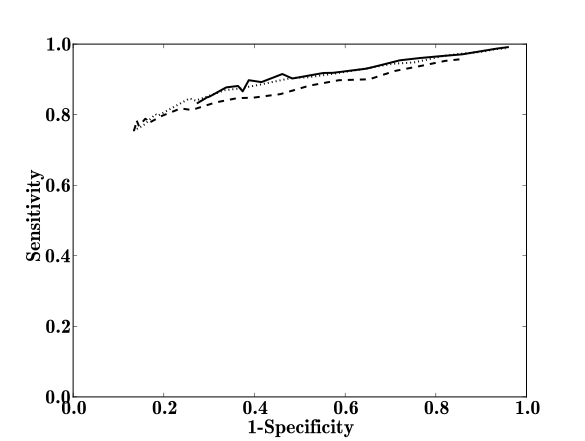
\includegraphics[width=.49\textwidth]{figs/amazon_pred_varying_mu}}
\subfigure[][]{\label{fig:1a}\includegraphics[width=.3\textwidth]{figs/clin_pred_varying_mu}}
%\subfloat[][\label{fig:1c}]{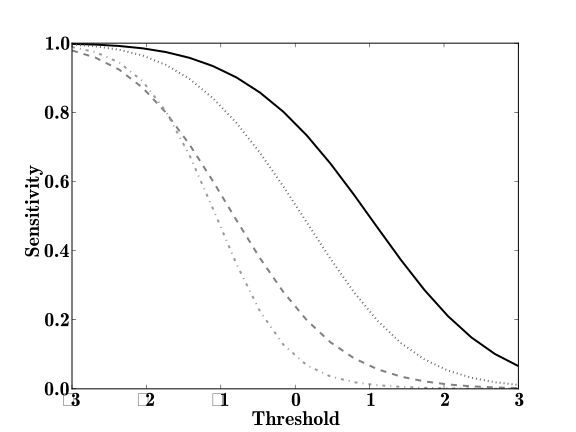
\includegraphics[width=.49\textwidth]{figs/sens_comparison_leafs}}
\subfigure[][]{\label{fig:1b}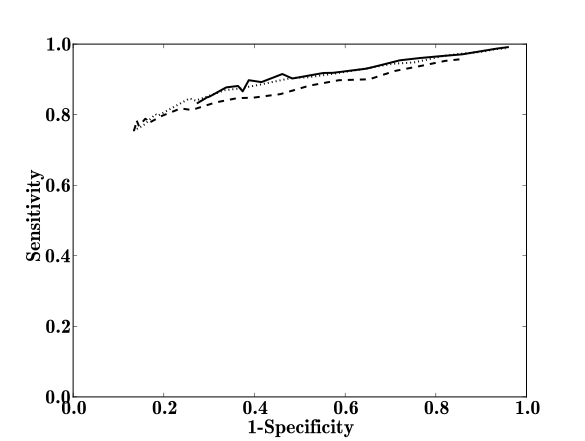
\includegraphics[width=.3\textwidth]{figs/amazon_pred_varying_mu}}
\subfigure[][]{\label{fig:clinical_roc}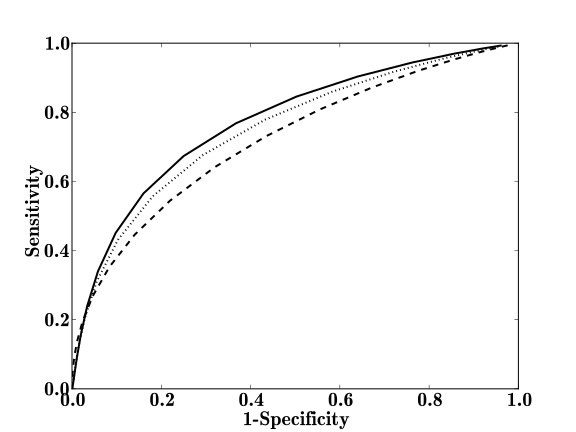
\includegraphics[width=0.3\textwidth]{figs/ROC_comparison_leafs}}
\caption{ROC curves for out-of-sample ICD-9 code prediction from patient free-text discharge records 
(\subref{fig:1a},\subref{fig:clinical_roc}). ROC curve for out-of-sample Amazon product category predictions from 
product free-text descriptions \subref{fig:1b}. Figures \subref{fig:1a} and \subref{fig:1b} are a function 
of the prior means of the regression parameters. Figure \subref{fig:clinical_roc} is a function of auxiliary variable threshold. In all figures, solid is 
HSLDA, dashed are independent regressors + sLDA (hierarchical 
constraints on labels ignored), and dotted is HSLDA fit by running LDA first then running 
tree-conditional regressions.}
\label{fig:main_results}
\end{center}
\end{figure}


The results in Figures~\ref{fig:1a} and \ref{fig:1b} suggest that in most cases
it is better to do full joint estimation of HSLDA.  An alternative
interpretation of the same results is that, if one is more sensitive to the
performance gains that result from exploiting the structure of the labels, then
one can, in an engineering sense, get nearly as much gain in label prediction
performance by first fitting LDA and then fitting a hierarchical probit
regression.  There are applied settings in which this could be advantageous.

\end{abstract}

\section{Introduction}
\label{sec:introduction}
There exist many sources of unstructured data that have been partially or
completely categorized by human editors.  In this paper we focus on
unstructured text data that has been, at least in part, manually
categorized.  Examples include but are not limited to webpages and curated
hierarchical directories of the same \citep{DMOZ}, product descriptions and
catalogs, %(e.g.~\citep{AMAZON} as available from \citep{SNAP})
and patient records %hospital treatment transcripts
and diagnosis codes assigned to them for bookkeeping and insurance purposes
(e.g.~hospital discharge summaries with 
International Classification of Disease 9th Revision, Clinical Modification
(ICD-9-CM) codes assigned \cite{ICD9}).  In this work we show how to combine
these two sources of information using a single model that allows one to
categorize new text documents automatically, suggest labels that might be
inaccurate, compute improved similarities between documents for information
retrieval purposes, and more. The models and techniques that we develop in
this paper are applicable in other data as well, namely, any unstructured
representations of data that have been hierarchically classified (e.g.,~image
catalogs with bag-of-feature image representations).

There are several challenges entailed in incorporating a hierarchy of labels
into the model. Given a large set of potential labels (often thousands), each
instance has only a small number of labels associated to it. There are no
naturally occurring negative labeling in the data, and the absence of a label
cannot always be interpreted as a negative labeling. 

Our work operates within the framework of topic modeling. Our approach learns
topic models of the underlying data and labeling strategies in a joint model,
while leveraging the hierarchical structure of the labels. For the sake of
simplicity, we focus on is-a hierarchies, but the model can be
applied to other hierarchies. We extend supervised latent Dirichlet
allocation (sLDA)~\cite{BleiMcAuliffe2008} to take advantage of hierarchical
supervision. We propose an efficient way to incorporate hierarchical
information into the model. We hypothesize that the context of labels within
the hierarchy provides valuable information about labeling. 

We demonstrate our model on large, real-world datasets in the clinical and web
retail domains. We observe that hierarchical information is valuable when
incorporated into the learning and improves our primary goal of multi-label
classification. Our results show that a joint, hierarchical model outperforms a
classification with unstructured labels as well as a disjoint model, where the
topic modeling and the hierarchical classification are carried out
independently of each other. 

The remainder of this paper is as follows. Section~\ref{sec:model}
introduces hierarchically supervised LDA (HSLDA), while
Section~\ref{sec:inference} details a sampling approach to inference in HSLDA. 
Section~\ref{sec:related_work} reviews related work, and
Section~\ref{sec:experiments} shows results from applying HSLDA to health care
and web retail data.  

%In this paper we describe the use of a topic model based on supervised
%latent Dirichlet allocation (sLDA) to identify topics within narrative
%discharge summaries and to automate the assignment of diagnostic codes,
%specifically International Classification of Disease 9th Revision,
%Clinical Modification (ICD-9-CM) codes. There are a number of advantages
%to this approach. First, manually coding diagnoses is a time-consuming
%and notoriously unreliable process. Many diagnoses are omitted in
%the final record, and a high error rate is found even in the principal
%diagnoses \citep{Surjan1999}.

%Our main contribution is to show how to utilize supervision in the form of
%hierarchical and (often) multiple labelings in a similar manner. Consider web
%retail data. Web retailers often have both a browse-able product hierarchy and
%free-text descriptions for all products they sell. The situation of each
%product in a product hierarchy (often multiply situated) constitutes a
%multiple, hierarchical labeling of the free-text product descriptions. We
%hypothesize that such hierarchical labels should, at least in theory, provide
%better supervision than the simpler unstructured labels previously considered.
%Results from applying our model to both medical record and web retail data
%suggests that this is likely the case. In particular, we observe gains in our
%primary goal of out-of-sample label prediction that result specifically from
%leveraging hierarchical supervision. 

%\begin{itemize}
%\item Benefits of combining human categorization information into ``topic models''
%\item LDA solved free text
%\item supervised LDA improves LDA (extra info) and allows new inference (predict links, etc.)
%\item amazon, freshdirect, netflix, dmoz, pandora (music genome)
%\end{itemize}


% Informatics journal paper
%
% Despite the growing emphasis on meaningful
%use of technology in medicine, many aspects of medical record-keeping
%remain a manual process. Diagnostic coding for billing and insurance
%purposes is often handled by professional medical coders who must
%explore a patient's extensive clinical record before assigning the
%proper codes. So while electronic health records (EHRs) should be
%adopted by most medical institutions within the next several years,
%largely due to the provisions of HITECH under the American Recovery
%and Reinvestment Act \citep{Blumenthal2009}, there has been little
%movement forward in automating medical coding.

%An automated process would ideally produce a more complete and accurate
%diagnosis lists. Also, this model will reveal information about the
%medical records themselves. For example, we may gain an understanding
%of what a specific code actually means in terms of clinical narratives.
%Similarly, viewing the distribution of topics over discharge summaries
%may reveal information about the latent structure of clinician documentation.
%Lastly, the sLDA model would provide a novel approach to dealing with
%the problem of high dimensionality when representing narrative text
%in a vector space specifically by reducing dimensions from an entire
%vocabulary of potentially tens of thousands of words to a set of several
%dozen topics.

%In this work we extend supervised latent Dirichlet allocation (sLDA)
%\cite{BleiMcAuliffe2008} to take advantage of hierarchical supervision.  sLDA
%is latent Dirichlet allocation (LDA) \cite{Blei2003} augmented with per
%document ``supervision'';  often taking the form of a single numerical or
%categorical ``label.''  More generally this supervision is just extra per
%document data;  for instance its quality or relevance (e.g.~online review
%scores), marks given to written work (e.g.~essay grades), or the number of
%times a web page is linked.  These labels are usually generatively modeled as
%having been conditionally drawn from some distribution that depends on the
%document-specific topic mixture.  It has been demonstrated that the signal
%provided by such supervision can result in better, task-specific document
%models and can also lead to good label prediction for out-of-sample data
%\cite{BleiMcAuliffe2008}. 




%\section{Background}


\section{Methods}
\label{sec:methods}

% generalize to arbitrary codes (not just ICD-9's

%
\begin{figure}[h]
%tbp] %  figure placement: here, top, bottom, or page
 \centering 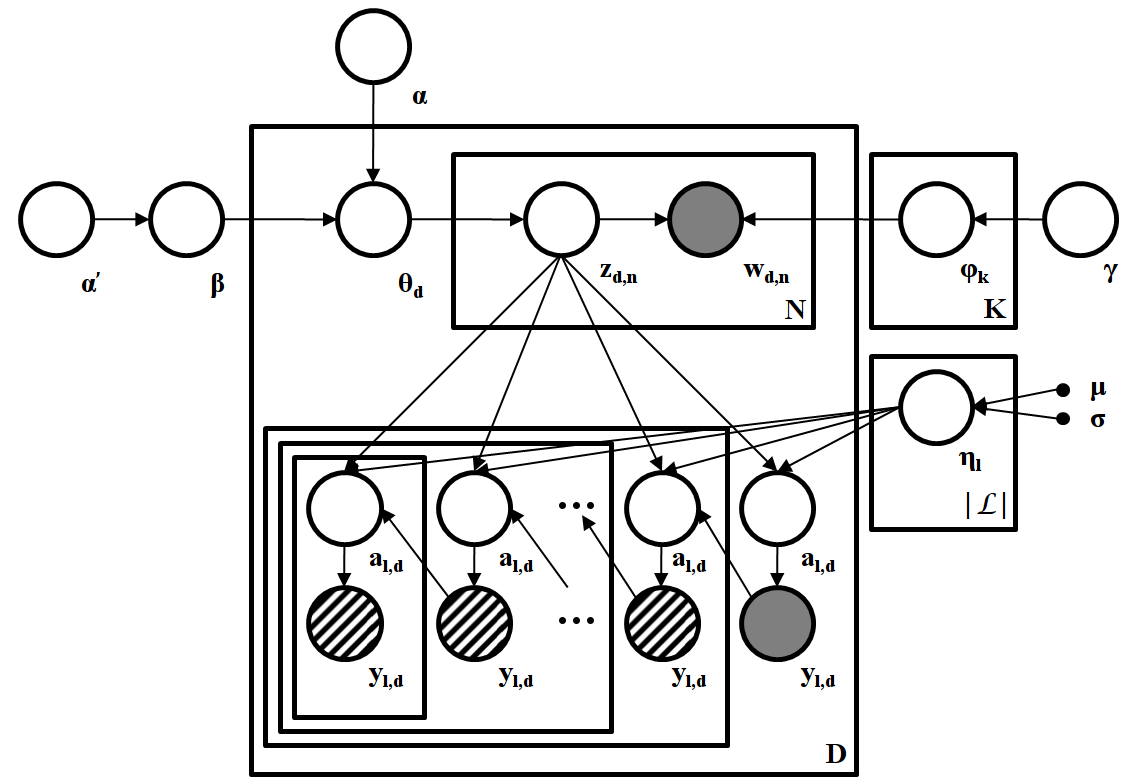
\includegraphics[scale=0.3]{Graphical_Model2} \caption{adapted sLDA model}


\label{fig:example} 
\end{figure}


Given the number of topics, K, and broad gamma priors on hyperparameters,
the generative process is as follows: 
\begin{enumerate}
\item For each topic, $k$:

\begin{enumerate}
\item Draw a distribution over words $\phi_{k}\sim Dir_{V}\left(\mathbf{1},\gamma\right)$ 
\end{enumerate}
\item For each ICD9 code, $c$, at all levels in the tree, $l$:

\begin{enumerate}
\item Draw regression coefficient $\eta_{i_{l,c}}\mid\sigma\sim\mathcal{N}_{K}\left(-\mathbf{1},\sigma\right)$ 
\end{enumerate}
\item Draw a prior over topic proportions $\beta\mid\alpha'\sim Dir_{K}\left(\mathbf{1},\alpha'\right)$ 
\item For each document, $d$:

\begin{enumerate}
\item Draw topic proportions $\theta_{d}\mid\beta,\alpha\sim Dir_{K}\left(\beta,\alpha\right)$ 
\item For each word, $n$:

\begin{enumerate}
\item Draw topic assignment $z_{n,d}\mid\theta_{d}\sim Mult_{K}\left(\theta_{d}\right)$ 
\item Draw word $w_{n,d}\mid z_{n,d},\beta_{1:K}\sim Mult_{V}\left(\beta_{z_{n}}\right)$ 
\end{enumerate}
\item For each level of the ICD-9 code tree, $l$:

\begin{enumerate}
\item For each ICD-9 code at this level, $c$:

\begin{enumerate}
\item Draw a latent variable \[
a_{d,i_{l,c}}\sim\begin{cases}
\mathcal{N}\left(\bar{z}^{T}\eta_{i_{l,c}},1\right), & y_{parent_{l,c}}=1\\
trunc\mathcal{N}^{-}\left(\bar{z}^{T}\eta_{i_{l,c}},1\right), & y_{parent_{l,c}}=-1\end{cases}\]
 where $\bar{z}=N^{-1}\sum_{n=1}^{N}z_{n}$ and $\mathcal{I}=\left\{ i_{0},i_{1},...,i_{\mathcal{L}}\right\} $
and $i_{l}=\left\{ i_{l,0},i_{l,1},...,i_{l,C_{l}}\right\} $
\item Draw a response variable $y_{d,i_{l,c}}\mid a_{d,i_{l,c}}\sim\begin{cases}
\begin{array}{c}
1,\\
-1,\end{array} & \begin{array}{c}
a_{d,i_{l,c}}>0\\
otherwise\end{array}\end{cases}$
\end{enumerate}
\end{enumerate}
\end{enumerate}
\end{enumerate}
The generative model for the ICD-9 codes is equivalent to a probit
regression model. In our case, the regression is conditional on the
parents according to the constraints of the ICD-9 code tree. The latent
variable utilized here is also known as an auxiliary variable.


\subsection{Posterior Inference}

Given an observation of a set of ICD-9 codes and a document, the posterior
distribution for the latent variables is given by Equation .

\begin{equation}
p\left(\theta,z_{1:N},\phi_{1:K},\eta_{i_{l,c}\in\mathcal{I}},a_{i_{l,c}\in\mathcal{I}},\beta,\alpha,\alpha',\gamma\mid w_{1:N},y_{i_{l,c}\in\mathcal{I}};\sigma,\lambda\right)\label{eq:Posterior}\end{equation}


\[
=\frac{p\left(\theta,z_{1:N},\phi_{1:K},\eta_{i_{l,c}\in\mathcal{I}},a_{i_{l,c}\in\mathcal{I}},\beta,\alpha,\alpha',\gamma,w_{1:N},y_{i_{l,c}\in\mathcal{I}};\sigma,\lambda\right)}{\int_{\theta,\phi,a,\eta,\alpha,\alpha',\beta,\gamma}\sum_{z}p\left(\theta,z_{1:N},\phi_{1:K},\eta_{i_{l,c}\in\mathcal{I}},a_{i_{l,c}\in\mathcal{I}},\beta,\alpha,\alpha',\gamma,w_{1:N},y_{i_{l,c}\in\mathcal{I}};\sigma,\lambda\right)}\]


The denominator for this distribution is the marginal probability
of the data and cannot be solved in closed form. This is often the
case in evaluating posterior distributions of non-trivial probabilistic
models. We will appeal to one of the common methods for approximating
posterior distributions in the face of intractable normalization factors:
Markov chain Monte Carlo (MCMC) sampling. Since in this model it is
possible to sample from the conditional distributions for all variables
we will use the Gibbs sampling algorithm to obtain an approximation
to this posterior. In particular, we will derive a collapsed Gibbs
sampler.


\subsection{Gibbs Sampling}

We derive a collapsed Gibbs sampler for this model, marginalizing
$\theta_{1:D}$ and $\phi_{1:K}$. For details regarding collapsing
in LDA models see \citet{Griffiths04}. To derive the Gibbs sampler
we evaluate the individual conditional probability distributions for
all unobserved variables.


\subsubsection{$p\left(z_{m,n}\mid\mathbf{z_{-\left(m,n\right)}},\mathbf{a},\mathbf{w},\mathbf{\eta},\alpha,\beta,\gamma\right)$}

For the purposes of sampling, we will be able to derive a representation
of the joint distribution isolating a particular latent variable,
$z$, for a word instance, $n$, in a document instance, $d$. The
conditional probability with respect to this latent variable is proportional
to the joint distribution of its markov blanket up to a constant.

\begin{equation}
p\left(z_{d,n}\mid\mathbf{z_{-\left(d,n\right)}},\mathbf{a},\mathbf{w},\mathbf{\eta},\alpha,\beta,\gamma\right)\propto p\left(z_{d,n},\mathbf{z_{-\left(d,n\right)}},\mathbf{a},\mathbf{w},\mathbf{\eta},\alpha,\beta,\gamma\right)\end{equation}


Due to the factorization of this model, we can rewrite the joint distribution
as the following:

\begin{equation}
\propto\prod_{i_{l,c}\in\mathcal{I}}p\left(a_{i_{l,c}}\mid\mathbf{z},\eta_{i_{l,c}}\right)p\left(z_{d,n},\mathbf{z_{-\left(d,n\right)}},\mathbf{a},\mathbf{w},\alpha,\beta,\gamma\right)\end{equation}


We isolate only terms that depend on $z_{m,n}$ and absorb all other
constant terms into the normalization constant \citep{Griffiths04}.

\begin{equation}
\propto\prod_{i_{l,c}\in\mathcal{I}}\exp\left\{ -\frac{\left(\bar{z}^{T}\eta_{i_{l,c}}-a_{i_{l,c}}\right)^{2}}{2}\right\} \left(n_{d,\left(\cdot\right)}^{k,-\left(d,n\right)}+\alpha\beta_{k}\right)\frac{n_{\left(\cdot\right),w_{d,n}}^{k,-\left(d,n\right)}+\gamma}{\sum_{v=1}^{V}\left(n_{\left(\cdot\right),w_{d,n}}^{k,-\left(d,n\right)}+\gamma\right)}\label{eq:z-likelihood}\end{equation}


Here, $n_{d,v}^{k,-\left(d,n\right)}$ represents the count of word
$v$ in document $d$ assigned to topic $k$ omitting the $(d,n)^{th}$
word count.

Given Equation \ref{eq:z-likelihood}, $p\left(z_{d,n}\mid\mathbf{z_{-\left(d,n\right)}},\mathbf{a},\mathbf{w},\mathbf{\eta},\alpha,\beta,\gamma\right)$
can be sampled through enumeration.


\subsubsection{$p\left(\eta_{i_{l,c}}\mid\mathbf{z}_{1:D},\mathbf{a};\sigma\right)$}

Given that $\eta_{i_{l,c}}$ and $a_{d,i_{l,c}}$ are distributed
normally, this posterior distribution is also normal. We evaluated
the model over various values of $\sigma$ where $\sigma=\left\{ 0.01,0.1,0.25,1,2\right\} $.

\begin{equation}
p\left(\eta_{i_{l,c}}\mid\mathbf{z}_{1:D},\mathbf{a};\sigma\right)=\mathcal{N}\left(\eta_{i_{l,c}}\mid\hat{\mu}_{i},\hat{\Sigma}_{i}\right)\end{equation}


\[
\hat{\mu}_{i}=\hat{\mathbf{\Sigma}}_{i}\left(-\mathbf{1}\sigma^{-1}+\bar{\mathbf{Z}}^{T}\mathbf{a}_{\left(\cdot\right),i_{l,c}}\right)\]


\[
\hat{\Sigma}_{i}^{-1}=\mathbf{I}\sigma^{-1}+\bar{\mathbf{Z}}^{T}\bar{\mathbf{Z}}\]



\subsubsection{$p\left(a_{d,i_{l,c}}\mid\mathbf{z},\mathbf{Y},\mathbf{\eta}\right)$
and \textmd{$p\left(y_{m,i}\mid\mathbf{a}\right)$}}

In the augmented probit regression model, the posterior distribution
of $a_{i_{l,c}}$ is distributed according to a truncated normal distribution
where the response variable is observed.

\begin{equation}
p\left(a_{d,i_{l,c}}\mid\mathbf{z},\mathbf{Y},\mathbf{\eta}\right)=\begin{cases}
trunc\mathcal{N}^{+}\left(a_{d,i_{l,c}}\mid\eta_{i}^{T}\bar{z,}\mathbf{1},y_{d,i_{l,c}}\right) & if\quad y_{d,i_{l,c}}=1\\
trunc\mathcal{N}^{-}\left(a_{d,i_{l,c}}\mid\eta_{i}^{T}\bar{z,}\mathbf{1},y_{d,i_{l,c}}\right) & if\quad y_{d,i_{l,c}}=-1\end{cases}\end{equation}


However, if $y_{d,i_{l,c}}$ is unobserved then $a_{d,i_{l,c}}$must
be sampled jointly with $y_{d,i_{l,c}}$ to ensure that the Markov
chain is ergodic. Suppose that $a_{d,i_{l,c}}$ is sampled to have
a negative value and $y_{d,i_{l,c}}$ is apporopriately sampled at
-1. Although there exist valid states where $a_{d,i_{l,c}}>0$ and
$y_{d,i_{l,c}}=1$, they will never be reached by such a Markov chain
since $p\left(a_{d,i_{l,c}}<0\mid y_{d,i_{l,c}}=-1\right)=1$ and
$p\left(y_{d,i_{l,c}}=-1\mid a_{d,i_{l,c}}<0\right)=1$. Therefore,
to ensure ergodicity, $a_{d,i_{l,c}}$and $y_{d,i_{l,c}}$ must be
sampled from the joint distribution as shown in Equation \ref{eq:Probit-Joint}.

\begin{equation}
p\left(a_{d,i_{l,c}},y_{d,i_{l,c}}\mid\mathbf{z},\mathbf{Y}_{-\left(d,i_{l,c}\right)},\mathbf{\eta}\right)\propto p\left(y_{i_{l,c}}\mid\mathbf{a},\mathbf{y}_{-\left(l,c\right)}\right)p\left(a_{d,i_{l,c}}\mid\mathbf{z},\mathbf{Y},\mathbf{\eta}\right)\end{equation}


\begin{equation}
p\left(y_{i_{l,c}}\mid\mathbf{a},\mathbf{y}_{-\left(l,c\right)}\right)=\delta\left(sign\left(a_{d,i_{l,c}}\right)=y_{i_{l,c}}\right)p\left(y_{i_{l,c}}\mid y_{parents_{l,c}}\right)\prod_{i_{\hat{l},\hat{c}}\in children_{l,c}}p\left(y_{i_{\hat{l},\hat{c}}}\mid y_{i_{l,c}}\right)\end{equation}


\begin{equation}
p\left(y_{i_{l,c}}=-1\mid y_{parent{}_{l,c}}\right)=\begin{cases}
1, & y_{parent_{l,c}}=-1\\
0.5, & y_{parent_{l,c}}=1\end{cases}\end{equation}


\[
p\left(a_{d,i_{l,c}},y_{d,i_{l,c}}\mid\mathbf{z},\mathbf{Y}_{-\left(d,i_{l,c}\right)},\mathbf{\eta}\right)\]


\begin{equation}
=\begin{cases}
\mathcal{N}\left(a_{d,i_{l,c}}\mid\bar{z}^{T}\eta_{i_{l,c}},1\right)p\left(y_{d,i_{l,c}}\mid a_{d,i_{l,c}}\right), & y_{parent_{l,c}}=1,\forall y_{i_{\hat{l},\hat{c}}}\in y_{children_{l,c}},y_{i_{\hat{l},\hat{c}}}=-1\\
trunc\mathcal{N}^{-}\left(a_{d,i_{l,c}}\mid\bar{z}^{T}\eta_{i_{l,c}},1\right)\delta\left(y_{d,i_{l,c}}=-1\right), & y_{parent_{l,c}}=-1\\
trunc\mathcal{N}^{+}\left(a_{d,i_{l,c}}\mid\bar{z}^{T}\eta_{i_{l,c}},1\right)\delta\left(y_{d,i_{l,c}}=1\right), & \exists y_{i_{\hat{l},\hat{c}}}\in y_{children_{l,c}}\setminus y_{i_{\hat{l},\hat{c}}}=1\\
0 & otherwise\end{cases}\end{equation}


where $\mathbf{Y}_{-\left(d,i_{l,c}\right)}$ denotes all of the response
variables excluding the response variable being sampled.


\subsubsection{$p\left(\beta\mid\mathbf{z},\alpha',\alpha\right)$}

In our model, we place a hierarchical Dirichlet prior over topic assignments.
This prior shares many features with the hierarchical Dirichlet process
and inference over this distribution proceeds in a very similar fashion.
This flexible distribution allows for an asymmetric prior over document
level distributions over topics \citet{WallachMiMc2009}.

Posterior inference was performed using the {}``direct assignment''
method of \citet{TehJorBea2006}.

\begin{equation}
\beta\sim Dir\left(m_{\left(\cdot\right),1},m_{\left(\cdot\right),2},\ldots,m_{\left(\cdot\right),K}\right)\end{equation}


\begin{equation}
p\left(m_{d,k}=m\mid\mathbf{z},\mathbf{m}_{-\left(d,k\right)},\beta\right)=\frac{\Gamma\left(\alpha\beta_{k}\right)}{\Gamma\left(\alpha\beta_{k}+n_{d,k}\right)}s\left(n_{d,k},m\right)\left(\alpha\beta_{k}\right)^{m}\end{equation}


where $s\left(n,m\right)$ represents stirling numbers of the first
kind.


\subsubsection{$p\left(\alpha;\lambda\right)$, $p\left(\alpha';\lambda\right)$,
$p\left(\beta;\lambda\right)$}

All hyperparameters were given broad gamma priors $\left(\lambda=\left\{ shape=2,scale=1000\right\} \right)$
and sampled via the Metropolis-Hastings algorithm.


\subsection{Prediction}


\section{Experiments}

\subsection{Data}

Our data set was gathered from the clinical data warehouse of NewYork
- Presbyterian Hospital. The data consisted of free-text discharge
summaries and their respective ICD-9 codes. A discharge summary is
a clinical report prepared by a physician or other health professional
at the conclusion of a hospital stay or series of treatments. The
note outlines the patient\textquoteright{}s chief complaint, diagnostic
findings, therapy administered, patient\textquoteright{}s response
to the chosen therapy, the treatment plan and the recommendations
upon discharge. The ICD-9 codes used to structure the discharge summary
data are part of a controlled terminology which is the international
standard diagnostic classification for epidemiological, health management,
and clinical purposes (http://www.who.int/classifications/icd/en/).
The codes are classified in a rooted-tree structure, with each edge
representing an is-a relationship between parent and child, such that
the parent diagnosis subsumes the child diagnosis. In the hospital,
ICD-9 codes are generated manually by trained medical coders, who
review all the information in the discharge summary. For the purposes
of sLDA, ICD-9 codes will be used as labels for discharge summaries.

We worked within the guidelines of the Health Insurance Portability
and Accountability Act (HIPAA), which protects patient privacy and
the security of potentially identifying medical material, known as
personal health information (PHI). HIPAA covers any information within
a medical record that was created, used, or disclosed during the course
of providing a health care service and that can be used to identify
an individual. Before beginning data processing, we generated a PHI-free
dataset (see Data Pre-processing below).


\subsection{Pre-Processing}

Patient discharge summaries and their associated ICD-9 diagnoses are
stored in two different places in the NewYork - Presbyterian data
warehouse, and so had to be linked together before being fed into
the sLDA algorithm. Each discharge note and set of diagnoses were
assigned a patient unique identifier (PUID) and a visit unique identifier
(VUID), allowing the two types of data to be linked.

Natural Language Processsing (NLP) techniques were used to process
the free-text discharge summaries. First, the Natural Language Toolkit
(http://www.nltk.org/) was used to tokenize the text. Next, feature
selection was performed using a term frequency - inverse document
frequency (TF-IDF) algorithm on the entire document set and sorting
the words by their TF-IDF values. The top 10,000 words were manually
evaluated to eliminate all potentially identifying information. Finally,
each discharge summary was converted to a bag-of-words, listing the
frequencies of the remaining, free of protected health information,
top 10,000 words.

Preparation of the diagnostic codes involved inference over the ICD-9
hierarchy. The is-a relationships of the hierarchy allowed us to make
two important assumptions. First, if a diagnosis was observed to be
present, all of its ancestors could be assumed to be present as well
(e.g., if a patient had malignant hypertension, it could be assumed
that they also had essential hypertension. Second, if a diagnosis
was observed to be absent, it could be assumed that all of its descendants
were also absent (e.g. if a patient did not have essential hypertension,
it could be assumed that they did not have malignant hypertension).
Unfortunately, ICD-9 code observations never include observations
of disease absence. ICD-9 codes are only documented when the condition
is observed to be present. Additionally, ICD-9 codes are known to
have relatively low sensitivity; conditions that are present are often
not documented in a set of ICD-9 codes (Surjan, 1999). Given these
facts, we made the following assumptions regarding each visit: recorded
diagnoses and their ancestors were labeled as true; diagnoses that
were observed at some time for a patient but not at the current visit
were labeled as unobserved; and diagnoses that had never been listed
for a patient were labeled as false for all of that patient\textquoteright{}s
visits. This last assumption captures the belief that parts of the
ICD-9 hierarchy that are never observed for a particular patient are
almost certain to be false. Additionally, for computational purposes,
we decided not to include an ICD-9 code at all if neither it nor one
of its descendants had been assigned to a patient in any of the records
in our dataset.


\subsection{ICD-9 Code Hierarchy}

Here, we augment the sLDA model such that the supervised signal is
distribution over the ICD-9 code tree, which is an is-a hierarchy
\citep{ICD9NCBO}. An is-a hierarchy is represented by the tree data
structure where each node has only a single parent and nodes cannot
be parents of ancestors (ie. there are no loops). In this particular
case, the ICD-9 code hierarchy is also partially a prefix trie where
the labels for certain nodes are prefixes for child nodes. Given that
this rule does not apply to all nodes in the hierarchy, we did not
use this feature to determine the structure of the hierarchy. Instead
we acquired a dataset that explicitly defined the relationships between
the nodes of the hierarchy \citep{ICD9NCBO}. In documentation of
ICD-9 codes for billing purposes, only a subset of the nodes can be
used, however the nodes higher in the hierarchy contain semantic information
about the categories of codes that are their descendants. For this
reason, we included these nodes in our model.



\subsection{Related Work}
\label{sec:related_work}
Latent dirichlet allocation (LDA) is a generative probabilistic model
of corpora that represents documents as a mixed membership bag-of-words.
Also known as topic models, these models infer the latent structure,
or topics, of documents in a corpus. Each document is represented
as a collection of words, generated from a set of topic assignments
(one for each word), where each topic assignment is drawn from a distribution
over topics \citep{Blei2003}.

This model, supervised latent dirichlet allocation (sLDA), builds
on LDA by incorporating an exponential family response variable. Although
there are many models for making predictions based on free text, sLDA
is unique in that it is a generative model, it represents documents
as a mixed-membership, and constrains the inference of the latent
structure of the documents by its predictability of the response variable.
In other words, sLDA infers topics such that the model is capable
of a high predictive likelihood for words in a document and the response
variable associated with a document. This approach has been shown
to outperform both LASSO (L1 regularized least squares regression)
and LDA followed by least squares regression \citep{BleiMcAuliffe2008}.

Other models - predicting document links, other supervised latent
variable models

% move to related work?
While there have been some attempts to automatically classify groups
of patients as a potential preliminary step to ICD-9 code assignment
\citep{Ruch2008,FreitasJunior2006,RibeiroNeto2001,Brown2006}, fully
automatic assignment of ICD-9 codes to medical text became a more
prevalent research topic only in the last few years. A subset of earlier
work proposed various methods on small corpora, based on a few specific
diseases \citep{Rao2003} but the most recent and promising work on
the subject was inspired by the 2007 Medical NLP Challenge: \textquotedblleft{}International
Challenge: Classifying Clinical Free Text Using Natural Language Processing\textquotedblright{}
(website). Most of the classification strategies included word matching
and rule-based algorithms. \citep{Goldstein2007,Crammer2007,Farkas2008}.
The data set given to the participants consisted only of documents
that were 1-2 lines each and all of the documents were radiology reports
- clearly limiting the scope of potential ICD-9 codes which could
be assigned. The only paper which has attempted to work with a document
scope as large as ours was the 2008 Lita et al publication \citep{Lita2008}.
Lita proposed support vector machine and bayesian ridge regression
methods to assign appropriate labels to the documents but did not
utilize the ICD-9 hierarchy to leverage more comprehensive predictions.

\subsection{Evaluation}

\section{Results}
\label{sec:results}

\begin{figure}[htbp]
\begin{center}
\subfigure[]{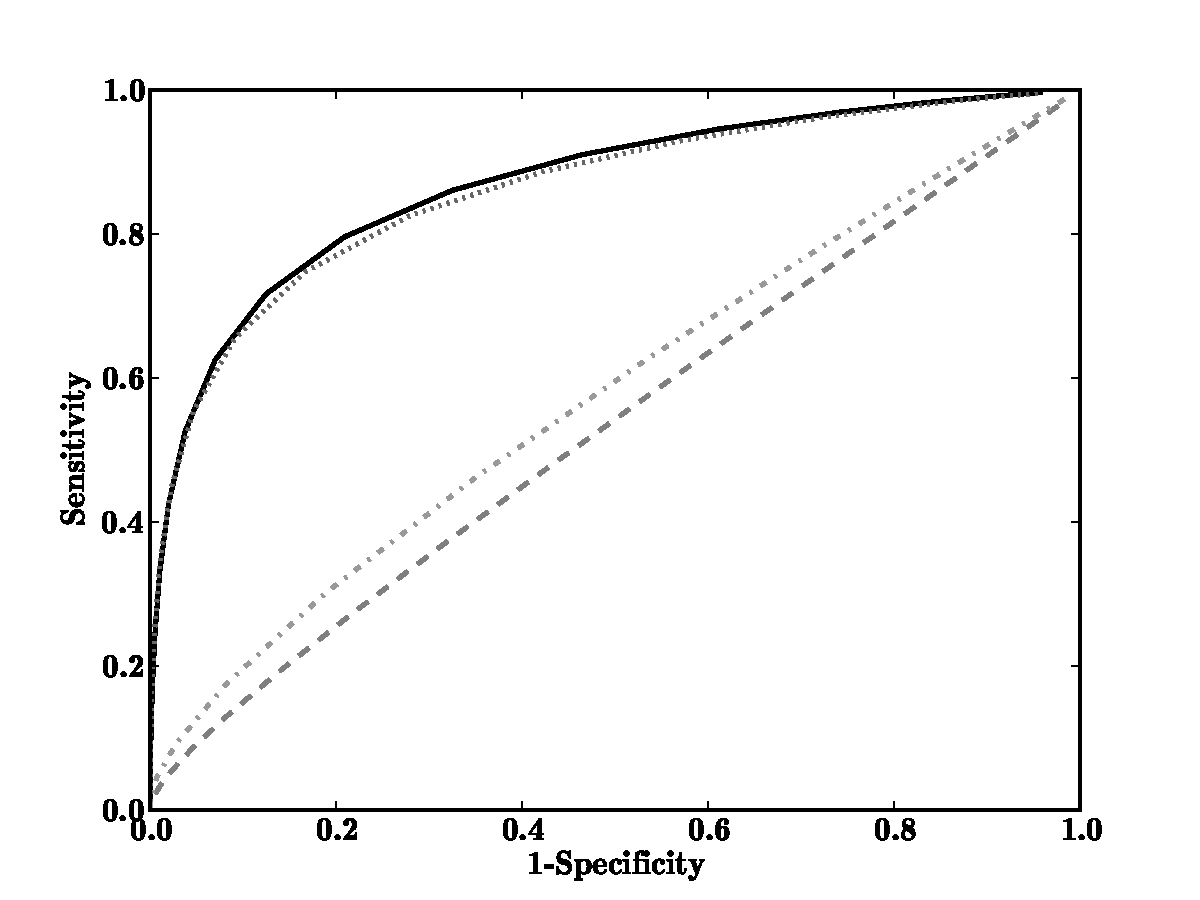
\includegraphics[width=.49\textwidth]{figs/ROC_comparison_ancestors}}
\subfigure[]{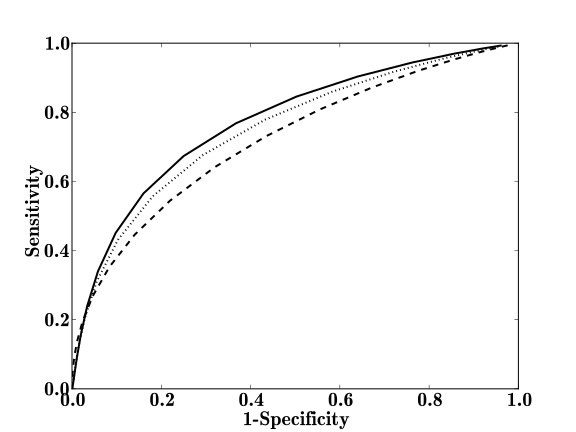
\includegraphics[width=.49\textwidth]{figs/ROC_comparison_leafs}}
\subfigure[]{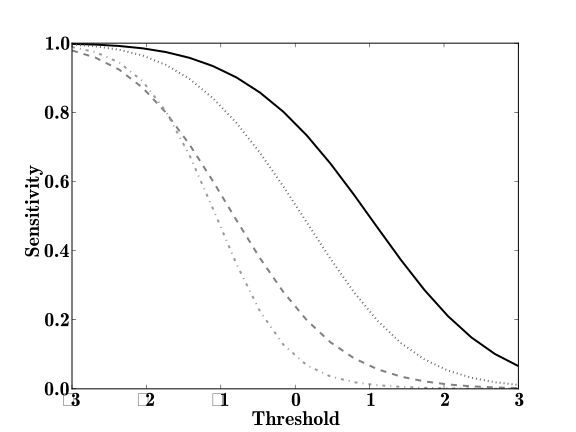
\includegraphics[width=.49\textwidth]{figs/sens_comparison_leafs}}
\subfigure[]{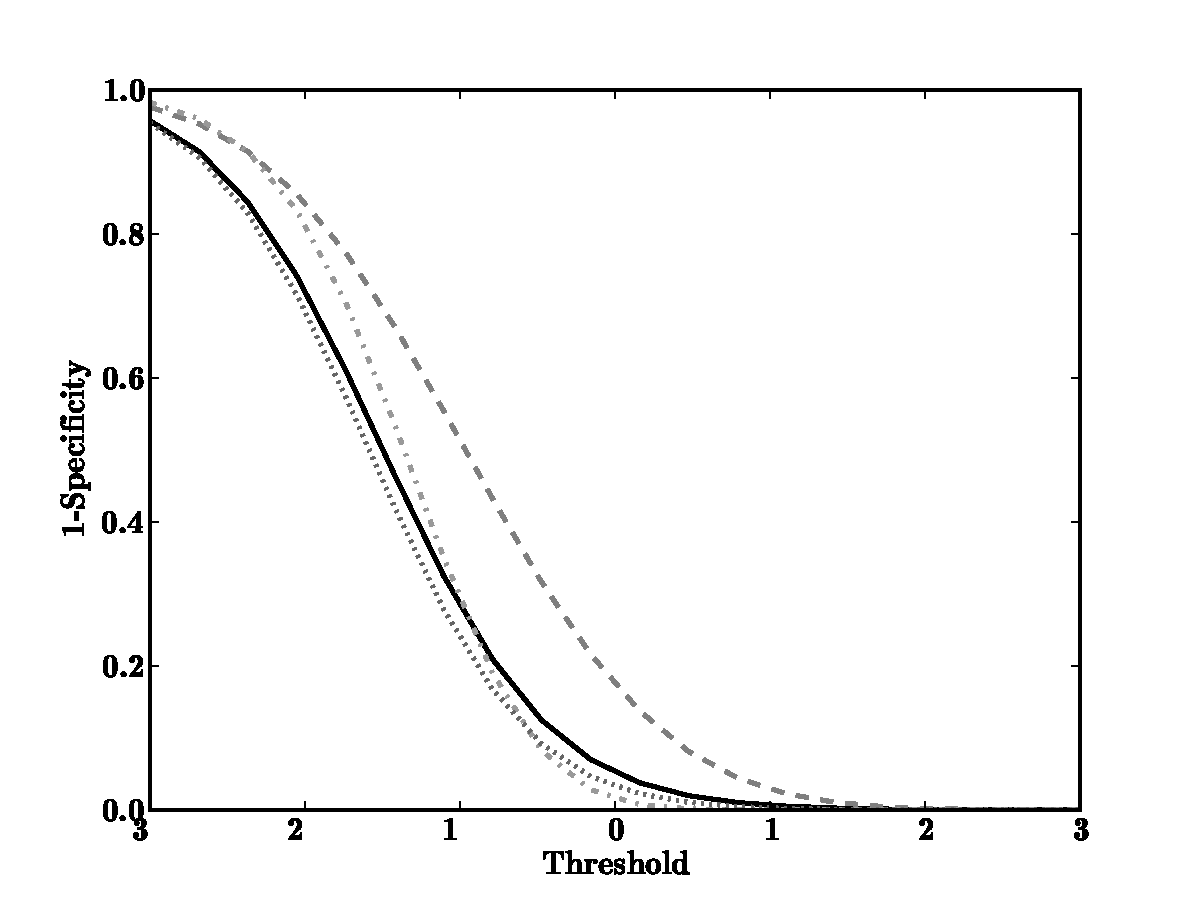
\includegraphics[width=.49\textwidth]{figs/one_m_spec_comparison_leafs}}
\caption{Out-of-sample ICD-9 code prediction from patient free-text discharge records.}
\label{fig:icd9}
\end{center}
\end{figure}


%We ran the Gibbs sampler for two days on 500 documents with 20 topics to learn the sLDA model which we then followed by a prediction of ICD-9 codes for 100 documents. The prediction resulted in 38 documents with at least 1 ICD-9 code assignment while some had over 200 assignments.


%\begin{figure}[h]%tbp] %  figure placement: here, top, bottom, or page
%   \centering
%   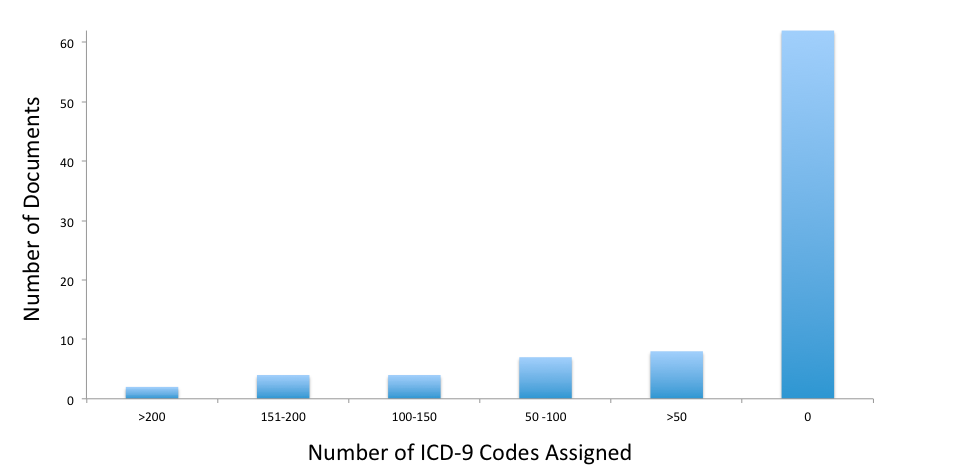
\includegraphics[width=4in]{number_of_codes_histogram} 
%   \caption{distribution of ICD-9 code assignments over all of the 100 documents predicted}
%   \label{fig:example}
%\end{figure}


%The accuracy of the prediction was tested against the actual ICD-9 codes in the EHR record for each discharge summary.  Different statistical measures were applied to asses the predictions.


%\begin{figure}[h]%tbp] %  figure placement: here, top, bottom, or page
%   \centering
%   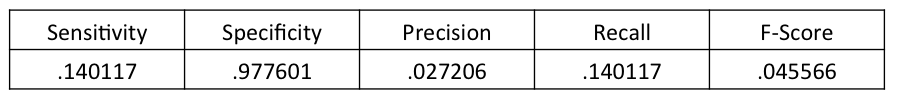
\includegraphics[width=4in]{signal_detection} 
%   \caption{sensitivity, specificity, precision, recall and F-measure.}
%   \label{fig:example}
%\end{figure}


%Although the sensitivty is not as high as we would have hoped, it is important to note that the sLDA was run on a very limited sample of documents (500) due to time constraints.  Additionally, the “gold standard” data used are actual hospital results which are very noisy given the incompleteness and introduction of human error.



\section{Discussion}
\label{sec:discussion}
%Despite the proliferation of LDA related models in recent years, one could argue that the true killer app for LDA has yet to be discovered.  LDA makes sense for information retrieval (IR) because  the learned latent topic vectors serve as good low-dimensional document representations, and, a posteriori similarity between such vectors can be used to compute the similarity of documents.  Unfortunately, computational considerations render this approach to IR impractical in most settings.

The SLDA model family, of which HSLDA is a member, can be understood in two different ways.  One way is to see it as a family of topic models that improve on the topic modeling performance of LDA via the inclusion of observed supervision.  Another way to see the family is as a set of models that can predict labels for bag-of-words data.  A large diversity of problems can be expressed as label prediction problems for bag-of-words data.  A surprisingly large amount of that kind of data possess structured labels, either hierarchically constrained or otherwise.  That HSLDA directly addresses this kind of data is a large part of the motivation for this work.   That it outperforms more straightforward approaches should be of interest to practitioners.

Variational Bayes has been the predominant estimation approach applied to sLDA models.  Hierarchical probit regression makes for tractable Markov chain Monte Carlo SLDA inference, a benefit that should extend to other sLDA models should probit regression be used for response variable prediction there too.  

The results in Figures~\ref{fig:1a} and \ref{fig:1b} suggest that in most cases it is better to do full joint estimation of HSLDA.  In alternative interpretation of the same results is that if one is more sensitive to the performance gains that result from exploiting the structure of the labels then one can, in an engineering sense, get nearly as much gain in label prediction performance by first fitting LDA and then fitting a hierarchical probit regression.  There are applied settings in which this could be advantageous.

Extensions to this work include unbounded topic cardinality variants and relaxations to different kinds of label structure.  Unbounded topic cardinality variants pose interesting inference challenges.  Utilizing different kinds of label structure is possible within this framework, but requires relaxing some of the simplifications we made in this paper for expositional purposes. 

%We have described a mixed membership model with hierarchical supervision. We have demonstrated this model in the context of document modeling with hierarchical multi-label supervision. Such a model is appropriate in domains where there are hierarchical constraints among the labels such as is the case in an IS-A hierarchy.

...

%\begin{itemize}
%\item what about the nonparametric version of this?
%\item discuss the broader goal, from the beginning of search engine time, to combine categorization and free text.  this, to our knowledge, is the first principled approach to doing so
%\end{itemize}

%We have proposed a new method for prediction of ICD-9 codes given a medical discharge summary note.  Our method explicitly takes advantage of the ICD-9 hierarchical IS-A relationships as well as the word distributions in each document.  We used Gibbs sampling for a supervised latent dirichlet allocation model to learn a distribution of words over twenty topics and their appropriate ICD-9 codes (response variable). The model was then tested on 100 discharge summaries for which the ICD-9 diagnoses were known.  The amount of ICD-9 codes produced for some discharge summaries was quite high because of the way the model worked with the IS-A hierarchy, highlighting the completeness of ICD-9 coding when using this sLDA model.  Overall, the model had extremely good specificity while the sensitivity was lower than anticipated.  Given our limited set of documents, and very noisy gold standard it would not be accurate to discount the use of sLDA in medical document classification and automatic coding.
%In future work, we plan to significantly expand the set of documents used to train the model (up to 15,000), as well as run several different iterations to learn the optimal topic number.  


%A more automated approach for coding patient visits with the ICD-9 hierarchy has great promise to  reduce health care costs and increase completeness of medical coded data.  We hope that this implementation of supervised LDA will serve as preliminary work for a much larger study with more documents in the future.


\begin{small} \bibliographystyle{plainnat} \bibliographystyle{plainnat}
\bibliographystyle{plainnat}
\bibliography{refs}


\end{small} 

\newpage{}


\subsection{Rao-Blackwellization}

To derive the Gibbs sampler in general, we integrate over the parameters
$\theta$ and $\phi_{1:K}$ resulting in the collapsed joint distribution
shown in Equations 5-8.

\begin{landscape} \centering % optional, probably makes it look better to have it centered on the page


\begin{small}

\begin{equation}
p\left(\theta,z_{1:N}\mid w_{1:N},y_{1:I},\phi_{1:K},\eta_{1:I},\alpha,\beta,\mu,\xi\right)=\frac{p\left(\theta\mid\alpha\right)\left(\prod_{n=1}^{N}p\left(z_{n}\mid\theta\right)p\left(w_{n}\mid z_{n},\phi_{1:K}\right)\right)\left(\prod_{k=1}^{K}p\left(\phi_{k}\mid\beta\right)\right)\left(\prod_{i=1}^{I}p\left(y_{i}\mid z_{1:N},\eta_{i},\xi\right)p\left(\eta_{i}\mid\mu\right)\right)}{\int_{\theta}p\left(\theta\mid\alpha\right)\sum_{k=1}^{K}\left(\prod_{n=1}^{N}p\left(z_{n}\mid\theta\right)p\left(w_{n}\mid z_{n},\phi_{1:K}\right)\right)\left(\prod_{k=1}^{K}p\left(\phi_{k}\mid\beta\right)\right)\left(\prod_{i=1}^{I}p\left(y_{i}\mid z_{1:N},\eta_{i},\xi\right)p\left(\eta_{i}\mid\mu\right)\right)d\theta}\end{equation}


\begin{equation}
\intop_{\theta}\intop_{\phi_{1:K}}p\left(\mathbf{Y},\mathbf{w},\mathbf{z},\mathbf{\theta},\mathbf{\phi},\mathbf{\eta},\alpha,\beta,\mu,\xi\right)d\theta d\phi_{1:K}=\intop_{\theta}\intop_{\phi_{1:K}}\prod_{k=1}^{K}p\left(\phi_{k};\beta\right)\prod_{m=1}^{M}\left\{ p\left(\theta_{m};\alpha\right)\prod_{n=1}^{N}\left[p\left(z_{m,n}\mid\theta_{m}\right)p\left(w_{m,n}\mid\phi_{z_{m,n}}\right)\right]\prod_{i=1}^{I}p\left(y_{m,i}\mid z_{m,1:N},\eta_{i},\xi\right)\right\} \prod_{i=1}^{I}p\left(\eta_{i};\mu\right)d\theta d\phi_{1:K}\end{equation}


\begin{equation}
p\left(\mathbf{Y},\mathbf{w},\mathbf{z},\mathbf{\eta},\alpha,\beta,\mu,\xi\right)=\prod_{i=1}^{I}\left[p\left(\eta_{i};\mu\right)\prod_{m=1}^{M}p\left(y_{m,i}\mid z_{m,1:N},\eta_{i},\xi\right)\right]\intop_{\phi_{1:K}}\prod_{k=1}^{K}p\left(\phi_{k};\beta\right)\prod_{m=1}^{M}\prod_{n=1}^{N}p\left(w_{m,n}\mid\phi_{z_{m,n}}\right)d\phi_{1:K}\intop_{\theta}\prod_{m=1}^{M}p\left(\theta_{m};\alpha\right)\prod_{n=1}^{N}p\left(z_{m,n}\mid\theta_{m}\right)d\theta\end{equation}


\begin{equation}
=\prod_{i=1}^{I}\left[p\left(\eta_{i};\mu\right)\prod_{m=1}^{M}p\left(y_{m,i}\mid z_{m,1:N},\eta_{i},\xi\right)\right]\prod_{k=1}^{K}\frac{\Gamma\left(\sum_{v=1}^{V}\beta_{v}\right)}{\prod_{v=1}^{V}\Gamma\left(\beta_{v}\right)}\frac{\prod_{v=1}^{V}\Gamma\left(n_{\left(\cdot\right),v}^{k}+\beta_{v}\right)}{\Gamma\left(\sum_{v=1}^{V}n_{\left(\cdot\right),v}^{k}+\beta_{v}\right)}\prod_{m=1}^{M}\frac{\Gamma\left(\sum_{k=1}^{K}\alpha_{k}\right)}{\prod_{k=1}^{K}\Gamma\left(\alpha_{k}\right)}\frac{\prod_{k=1}^{K}\Gamma\left(n_{m,\left(\cdot\right)}^{k}+\alpha_{k}\right)}{\Gamma\left(\sum_{k=1}^{K}n_{m,\left(\cdot\right)}^{k}+\alpha_{k}\right)}\end{equation}


\begin{equation}
=\prod_{i=1}^{I}\left[\mathcal{N}\left(\eta_{i}\mid\mu,1\right)\prod_{m=1}^{M}h\left(y\right)\exp\left\{ \left(\eta_{i}^{T}\bar{z}\right)y-A\left(\eta_{i}^{T}\bar{z}\right)\right\} \right]\prod_{k=1}^{K}\frac{\Gamma\left(\sum_{v=1}^{V}\beta_{v}\right)}{\prod_{v=1}^{V}\Gamma\left(\beta_{v}\right)}\frac{\prod_{v=1}^{V}\Gamma\left(n_{\left(\bullet\right),v}^{k}+\beta_{v}\right)}{\Gamma\left(\sum_{v=1}^{V}n_{\left(\bullet\right),v}^{k}+\beta_{v}\right)}\prod_{m=1}^{M}\frac{\Gamma\left(\sum_{k=1}^{K}\alpha_{k}\right)}{\prod_{k=1}^{K}\Gamma\left(\alpha_{k}\right)}\frac{\prod_{k=1}^{K}\Gamma\left(n_{m,\left(\bullet\right)}^{k}+\alpha_{k}\right)}{\Gamma\left(\sum_{k=1}^{K}n_{m,\left(\bullet\right)}^{k}+\alpha_{k}\right)}\end{equation}


\end{small} \end{landscape}
\end{document}

%\begin{align}
%p\left(\theta,z_{1:N},\phi_{1:K},\eta_{i_{l,c}\in\mathcal{I}},a_{i_{l,c}\in\mathcal{I}},\beta,\alpha,\alpha',\gamma\mid w_{1:N},y_{i_{l,c}\in\mathcal{I}};\sigma,\lambda\right) & =\\
% & \frac{p\left(\alpha,\alpha',\gamma;\lambda\right)p\left(\beta\mid\alpha'\right)p\left(\theta\mid\beta,\alpha\right)\left(\prod_{n=1}^{N}p\left(z_{n}\mid\theta\right)p\left(w_{n}\mid z_{n},\phi_{1:K}\right)\right)\left(\prod_{k=1}^{K}p\left(\phi_{k}\mid\gamma\right)\right)\left(\prod_{i_{l,c}\in\mathcal{I}}p\left(y_{i_{l,c}}\mid z_{1:N},\eta_{i_{l,c}}\right)p\left(\eta_{i_{l,c}};\sigma\right)\right)}{\int_{\alpha,\alpha',\gamma}p\left(\alpha,\alpha',\gamma;\lambda\right)p\left(\beta\mid\alpha'\right)\int_{\theta}p\left(\theta\mid\beta,\alpha\right)\sum_{k=1}^{K}\left(\prod_{n=1}^{N}p\left(z_{n}\mid\theta\right)p\left(w_{n}\mid z_{n},\phi_{1:K}\right)\right)\left(\prod_{k=1}^{K}p\left(\phi_{k}\mid\gamma\right)\right)\left(\prod_{i_{l,c}\in\mathcal{I}}p\left(y_{i_{l,c}}\mid z_{1:N},\eta_{i_{l,c}}\right)p\left(\eta_{i_{l,c}};\sigma\right)\right)}\end{align}
